%% measurement methodology appendix 

%\FloatBarrier
%\subsubsection{Measurement methodology and data analysis}
In order to measure the ambient seismic background low noise broadband seismometers are required. All seismic measurements were carried out using two measurement stations, each station consists of a Trillium 240 (T240) accelerometer and a data acquisition system. The T240 is a broadband low noise seismometer with a flat velocity response from 4 mHz to 35 Hz and a self noise below the low noise model from 0.01 to 10 Hz. Each seismometer is placed on top of a granite tile that is fixed to the solid rock floor with tile glue. A thermal and acoustic insulation cover is then placed over the seismometer. The read-out of the seismometers is done with a portable data acquisition system consisting of a 19 inch rack mounted computer with a National Instruments 18 bit DAQ card, a low noise amplifier, a battery UPS and a power supply to both the seismometer and amplifier. The seismometer produces a sensitive measurement of the ground velocity in 3 directions (north, east and vertical) and a number of diagnostic signals. The velocity channels are amplified by a factor of 105 to increase the resolution of the read-out system and passed through a low-pass filter with a -3 dB point at 30 Hz. The sampling rate is 128 Hz and every 128 seconds of data are written away into a single ascii data file by using a custom made LabView program.

The measurement noise of the seismic station is dominated by the self-noise of the T240 and the electronic noise from the pre-amplifer. The latter can be decomposed into voltage, thermal and current noise contributed by the first stage operational amplifier (op-amp), and ADC or quantization noise at the digitizer. The electronic noise at the input of the amplifier, can be modeled given the following equations~\cite{Rodgers1994};
\begin{eqnarray}
\label{eq:elecnoise1}
E_{nn} &=& V_{00}\left(\frac{f_{cv}}{f}+1\right)+ I_{00}\left(\frac{f_{ci}}{f}+1\right)r_p^2+4kTr_p+\frac{D_{nn}}{A_G^2}  \hspace{0.5 cm} V^2/\mbox{Hz} \\
D_{nn} &=& \left(\frac{2A}{2^n}\right)^2\frac{1}{12f_N} \hspace{0.5 cm} V^2/\mbox{Hz},
\label{eq:elecnoise3}
\end{eqnarray}

where, $f_{cv}$ and $f_{ci}$, are the corner frequencies of op-amp voltage and current noise, $V_{00}$ and $I_{00}$, the high frequency levels of op-amp voltage and current noise power spectral density. Boltzmann's constant is denote $k$, $T$ is the temperature in Kelvin and appears in the op-amp Johnson or thermal noise contribution, $r_p$ is the parallel combination of $r_c$ and $r_d$ and are the seismometer and shunt resistance respectively. Finally, the maximum amplitude of ADC input is $A$, $A_G$ is the amplifier gain, $f_N$ is the Nyquist frequency (related to the sampling frequency, $f_N = f_s/2$), and $n$ the number of bits in the ADC. 

\begin{table}[h]
\center
\begin{tabular}{| l | c | c | c | c | c |}
\hline
\multicolumn{6}{|l|}{Op-amp parameters} \\
\hline
Type & $V_{00}$[$V^2$/Hz] & $f_{cv}$ [Hz] & $I_{00}$ [$A^2/$Hz] &$f_{cv}$ [Hz] & $A_G$ gain \\
\hline
INA128  &	$6.4 \cdot 10^{17} $& 10 & $9 \cdot 10^{-26} $ & 200 & 105 \\
\hline
\multicolumn{6}{|l|}{ADC parameters} \\
\hline
Type & A [V] & Bits $n$ & $f_N$ [Hz] & $r_c$ [$\Omega$] & $r_d$ [$\Omega$] \\
\hline
NI 6289 & 10 & 18 & 64 & 300 & 10k \\
\hline
\end{tabular}
\caption{Op-amp and ADC parameters used in the self-noise model calculations. }
\label{tab:ampnoise}
\end{table}


Fig.~\ref{Fig:Seis_noise} shows the outcome of Eq.~(\ref{eq:elecnoise1}) with the seismic stations parameters (given in Tab.~\ref{tab:ampnoise}) along with the T240 self-noise provided by the manufacturer and the measured ADC and amplifier noise. The latter was obtained by short-circuiting the amplifier input with a impedance equal to that of the seismometer output ($300~\Omega$). The ADC and amplifier noise is consistent with the expected values from Eq.~(\ref{eq:elecnoise1}), the dip in measured noise above 10 Hz is due to the seismometer response function. This suggests that the electronic noise is dominated by ADC noise. The total noise of the system stays below the NLNM between 0.03 and 8 Hz and is dominated by the T240 self-noise, except between 0.3 and 20 Hz where the amplifier electronic noise plays a dominate role.
\begin{figure}[h]
	\begin{center}
		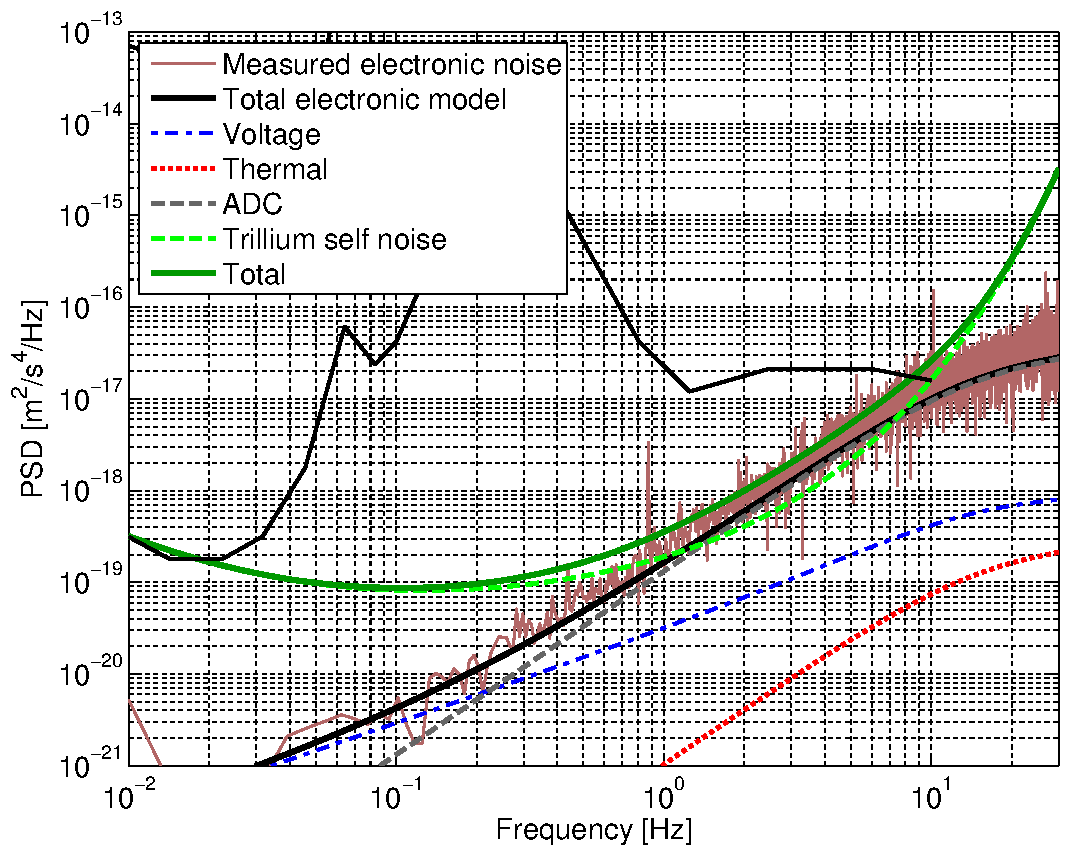
\includegraphics[width=0.65\textwidth]{./Appendices/Figures/T240_noise_contributions.pdf}\hspace{1pc}%
		\caption{Noise characterization of the seismic data acquisition system. The main contributor to the electronica noise is ADC noise calculated from Eq.~(\ref{eq:elecnoise1}) and voltage noise from the first stage op-amp of the pre-amplifier. The Trillium 240 self-noise is provided by the manufacturer. The total noise is below the low noise model between 0.03 and 8 Hz.}
		\label{Fig:Seis_noise}
	\end{center}
\end{figure}

The on-site seismic measurements were made over a period of 5 to 6 days. Care was taken to ensure that the measurement time includes at least a weekend and a number of week days. To characterize seismic measurements the amplitude of each frequency component of the velocity channels are calculated using Fourier analysis. In all of the following results a fast Fourier transform (FFT) was performed on stretches of 128 seconds of data to obtain an power spectral density (PSD) in (m$^2$/s$^4$)/Hz. The PSDs are averaged over a period of half an hour. Averaged PSD values are smoothed by taking the average of the PSD values in a constant relative bandwidth of 1/10 decade. (So for low frequencies the averaging is over only a few points, for high frequencies the averaging is over many more points). For comparison the new high and low noise models are also plotted. These models indicate theoretical  values for extremely high and extremely low seismic noise locations respectively. Spectral variation plots are used here to not only show the amplitude of the seismic signal but also how much time, as a percentage, is spent at a certain level. This is indicated by the color of the plot. The spectral variation plots also contain three solid line plots to indicate the mode and the 90 and 10~\% levels. The mode is the most common PSD value in each frequency bin, and 90 and 10~\% levels indicate the point under which the PSD will stay for 90 or 10~\% of the time, respectively. 